\documentclass[12pt, oneside]{article}
\usepackage[letterpaper, margin=1in, headsep=0.5in]{geometry}
\usepackage[english]{babel}
\usepackage[utf8]{inputenc}
\usepackage{amsmath}
\usepackage{amsfonts}
\usepackage{amssymb}
\usepackage{tikz}
\usetikzlibrary{quotes, angles}
\usepackage{graphicx}
%\usepackage{pgfplots}
%\pgfplotsset{width=10cm,compat=1.9}
%\usepgfplotslibrary{statistics}
%\usepackage{pgfplotstable}
%\usepackage{tkz-fct}
%\usepackage{venndiagram}

\usepackage{fancyhdr}
\pagestyle{fancy}
\fancyhf{}
\rhead{\thepage \\Name: \hspace{1.5in}.\\}
\lhead{BECA / Dr. Huson / 10th Grade Geometry\\* 29 October 2018}

\renewcommand{\headrulewidth}{0pt}

\begin{document}
\subsubsection*{Homework: Construct a median, transversal practice}
Use only a compass and straightedge for these classical constructions.
  \begin{enumerate}

  \item Construct the midpoint $M$ of $\overline{BC}$ by using the perpendicular bisector construction. Draw $\overline{AM}$, a \emph{median} of $\triangle ABC$.\\
  Spicy: Construct the other two medians, and hence, the centroid.
    \vspace{1cm}
    \begin{center}
    \begin{tikzpicture}
      \draw [<->, thick] (0,0)--(7,0)--(6,4)--cycle;
      \draw [fill] (0,0) circle [radius=0.05] node[left]{$A$};
      \draw [fill] (7,0) circle [radius=0.05] node[right]{$B$};
      \draw [fill] (6,4) circle [radius=0.05] node[above right]{$C$};
    \end{tikzpicture}
  \end{center} \vspace{1.5cm}

  \item Given two parallel lines and a transversal, as shown. Apply the theorem ``If a transversal intersects two parallel lines, then corresponding angles are congruent."
  \begin{center}
  \begin{tikzpicture}
    \draw [<->, thick] (1,2)--(9,2);
    \draw [<->, thick] (0,0)--(8,0);
    \draw [<->, thick] (4,-1)--(5.5,3);
    \node at (4.5,0.3) [left]{$5$};
    \node at (4.5,0.3) [right]{$6$};
    \node at (4.3,-0.3) [left]{$7$};
    \node at (4.3,-0.3) [right]{$8$};
    \node at (5.2,2) [above left]{$1$};
    \node at (5.2,2) [above right]{$2$};
    \node at (5,2) [below left]{$3$};
    \node at (5,2) [below right]{$4$};
  \end{tikzpicture}
  \end{center}
    \begin{enumerate}
      \item State the angle corresponding with $\angle 7$. \bigskip
      \item Given $m\angle 6 = 80^\circ$ and $m\angle 2 = 2x^\circ$. Find $x$. \bigskip
      \item Given $m\angle 5 = 100^\circ$. Find $m\angle 3$.
    \end{enumerate}

\newpage
\item Given the quadrilateral $RECT$ with $R(-4,1)$, $E(8,1)$, $C(8,6)$, and $T(-4,6)$.
\begin{enumerate}
  \item Plot and label $RECT$ on the grid.
  \item Using the distance formula, calculate the length of the two diagonals $RC$ and $ET$.
  \item Theorem: If the diagonals of a quadrilateral are congruent, then it is a rectangle.\\[0.5cm]
  Prove that $RECT$ is a rectangle.
\end{enumerate}

\begin{center} %4 quadrant regents grid w T-Chart
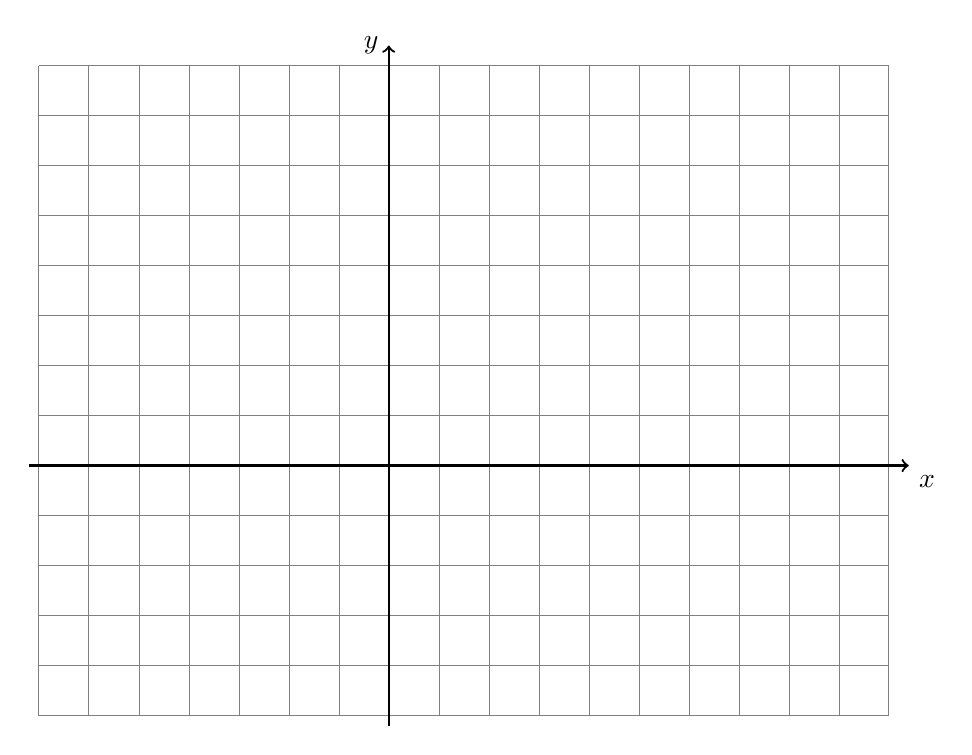
\begin{tikzpicture}[scale=.635]
  \draw [help lines] (-7,-5) grid (10,8);
  \draw [thick, ->] (-7.2,0) -- (10.4,0) node [below right] {$x$};
  \draw [thick, ->] (0,-5.2)--(0,8.4) node [left] {$y$};
\end{tikzpicture}
\end{center}


\end{enumerate}
\end{document}
